% Licensed to the Apache Software Foundation (ASF) under one or more
% contributor license agreements. See the NOTICE file distributed with
% this work for additional information regarding copyright ownership.
% The ASF licenses this file to You under the Apache License, Version 2.0
% (the ``License''); you may not use this file except in compliance with
% the License. You may obtain a copy of the License at
%
% http://www.apache.org/licenses/LICENSE-2.0
%
% Unless required by applicable law or agreed to in writing, software
% distributed under the License is distributed on an ``AS IS'' BASIS,
% WITHOUT WARRANTIES OR CONDITIONS OF ANY KIND, either express or implied.
% See the License for the specific language governing permissions and
% limitations under the License.

\begin{changemargin}{1.5in}{0in}

\section{Overview}

The MetaCarta GTS appliance indexes documents and allows users to
search these documents based on both keywords and geographic
references. The MetaCarta Meridio Connector Field Test allows system
administrators to configure connections to Meridio repositories and
define jobs to maintain synchronization between the repositories and
the GTS index.

This document specifies the means for connecting to these repositories,
indexing files from these repositories, and maintaining connections to
these repositories.

\subsection{Assumptions}

This document assumes you have a basic level of familiarity with GTS
appliance administration. This document also assumes that you have
a basic understanding of the repositories to which you are trying to
connect. If you need more information about the MetaCarta GTS appliance,
please read the \documentref{MetaCarta GTS Administrator's Guide} stored
on the appliance at \dirpath{/usr/share/doc/metacarta/AdminGuide.pdf}. For
more information about Meridio, please see your Meridio documentation
or Meridio administrator.

Throughout this document, we assume that your appliance is named \\
\url{metacarta.example.com}. 

\section{Installation}

The Meridio Connector must be used with the MetaCarta Connector
Framework, described in the \documentref{Metacarta Connector
Guide}. If you already have the Connector Framework installed, you can
install the Meridio Connector.  The Meridio Connector is
available as a field-test addon ISO file from from Metacarta. Use the
following steps to install the Meridio Connector to your appliance:

\begin{enumerate}

\item Confirm that the system is running correctly using
\command{check\_system\_health}.

\item Copy the disc image and md5sum supplied by MetaCarta to the
\dirpath{/isos} directory on your appliance. Rename the ISO file to
\dirpath{addon-mer-conn.iso} when you copy it to your appliance.

\item Check the md5sum of the ISO file using the \command{md5sum} command.

\item Install the iso using the following command:

\command{upgrade\_control install /isos/addon-mer-conn.iso}

The appliance will reboot once the installation is complete.

\item Upgrade your license file, if necessary, as described in
\documentref{MetaCarta Appliance Administrator's Guide}. You may need
to contact MetaCarta Customer Service to obtain the appropriate
license file. (Please see page \pageref{SupportContact} for contact
information.)
 
\end{enumerate}


\subsection{MetaCarta Meridio Web Service Installation}\label{SWService}

The MetaCarta Meridio Web Service must be installed on a Meridio
server running .NET framework version 1.1. The
Meridio Web Service installer at  
\dirpath{/usr/share/metacarta/MetaCarta}\linebreak\dirpath{MeridioWebServiceInstaller.zip},
is installed on your appliance when you install the Meridio Connector.
You will need to copy this archive to your Meridio
server and then unpack it. Read the file \dirpath{readme.txt} from the
unpacked archive, and follow the directions in the file. The package
also contains several executable files allowing you to install,
upgrade, or remove the Meridio Web Service. The detailed commands are
described in the \dirpath{readme.txt} file.

\section{Configuration}

\subsection{Access to the Connector}

The administrator to the Meridio Connector % Licensed to the Apache Software Foundation (ASF) under one or more
% contributor license agreements. See the NOTICE file distributed with
% this work for additional information regarding copyright ownership.
% The ASF licenses this file to You under the Apache License, Version 2.0
% (the ``License''); you may not use this file except in compliance with
% the License. You may obtain a copy of the License at
%
% http://www.apache.org/licenses/LICENSE-2.0
%
% Unless required by applicable law or agreed to in writing, software
% distributed under the License is distributed on an ``AS IS'' BASIS,
% WITHOUT WARRANTIES OR CONDITIONS OF ANY KIND, either express or implied.
% See the License for the specific language governing permissions and
% limitations under the License.

must have
access to the web interface at
\url{http://metacarta.example.com/crawler/}. In the default appliance
security setup, you must have a Basic Authentication account
configured for access to the Connector web interface at
\url{http://metacarta.example.com/crawler/}.  If you are not an appliance
administrator, please ask the appliance administrator to give you such
an account.

An appliance administrator can create an account with access to the
ingestion interface (in this case, username {\tt fred} and password
{\tt ginger}) by running the following command on the appliance:

\begin{console}
metacarta:\~{}\$ basic\_auth\_control add ingest\_users fred:ginger 
\end{console}

Depending on how you have configured authentication using the
\command{auth\_control} tool, you may need to make changes other than
adding yourself to the ingest\_users group. For more information on
security configuration and \command{auth\_control}, see the Security
Administration section of the \documentref{MetaCarta Appliance
Administrator's Guide}.


\section{Collecting Documents From Repositories} % Retitle this, yo.

The Connector Framework manages retrieving documents from different
repositories through \emph{jobs}. Jobs can be scheduled to run
regularly; each job connects to a single repository using a particular
set of credentials. Each job is tied to a \emph{repository
connection}. Repository connections contain information allowing the
connector framework to connect to a given repository --- that is, a
given Meridio server. Each repository connection is also tied
to an \emph{authority connection}. These authority connections manage
document security, making sure that when files have been indexed on
your GTS appliance, only authorized users are able to view them as
search results. Before you can create a job, you must create a
repository connection for the job to use. Each repository connection
should be set up with an appropriate authority, in this case a
Meridio authority connection. 

\subsection{Creating Authority Connections}

To create an authority connection, first go to the
main Connector Framework Administration interface at
\url{metacarta.example.com/crawler/}.  By default, your username and
password are the Ingestion Basic Auth username and password defined
earlier. 

You will see a sidebar like the one to the left. Click on ``List
Authority Connections'' and then you will be presented with the
list of authority connections. Click ``Add a new connection.''
You will see the following:

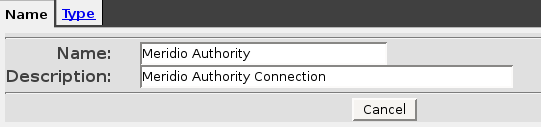
\includegraphics[width=300pt]{mer-edit-auth-tab1}

This is the first tab of the tabbed interface you will use to edit
authority connections. The next tab is as follows:

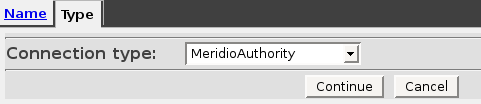
\includegraphics[width=300pt]{mer-edit-auth-tab2}


% Licensed to the Apache Software Foundation (ASF) under one or more
% contributor license agreements. See the NOTICE file distributed with
% this work for additional information regarding copyright ownership.
% The ASF licenses this file to You under the Apache License, Version 2.0
% (the ``License''); you may not use this file except in compliance with
% the License. You may obtain a copy of the License at
%
% http://www.apache.org/licenses/LICENSE-2.0
%
% Unless required by applicable law or agreed to in writing, software
% distributed under the License is distributed on an ``AS IS'' BASIS,
% WITHOUT WARRANTIES OR CONDITIONS OF ANY KIND, either express or implied.
% See the License for the specific language governing permissions and
% limitations under the License.

\begin{picture}(1,1)
  \put(-100,15){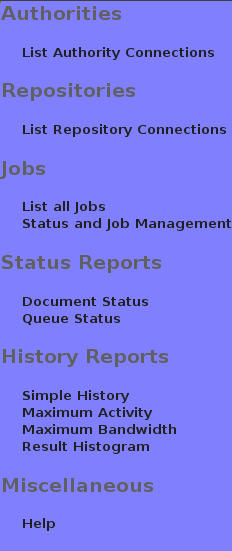
\includegraphics[width=80pt]{crawler-sidebar}}
\end{picture}



In the first two tabs you must provide a name, description, and
authority type for your new authority connection. The name should be
unique, as you will use it to select this connection later when making
repository connections. The description should explain the authority
connection to you or another administrator. The authority type is the
type of authority to which you will connect, in this case a
MeridioAuthority.

Once you have filled in those tabs, click continue, and then you must
fill in the following extra tabs specific to Meridio Authority
Connections:

% Licensed to the Apache Software Foundation (ASF) under one or more
% contributor license agreements. See the NOTICE file distributed with
% this work for additional information regarding copyright ownership.
% The ASF licenses this file to You under the Apache License, Version 2.0
% (the ``License''); you may not use this file except in compliance with
% the License. You may obtain a copy of the License at
%
% http://www.apache.org/licenses/LICENSE-2.0
%
% Unless required by applicable law or agreed to in writing, software
% distributed under the License is distributed on an ``AS IS'' BASIS,
% WITHOUT WARRANTIES OR CONDITIONS OF ANY KIND, either express or implied.
% See the License for the specific language governing permissions and
% limitations under the License.

\subsubsection{Configuring a Meridio Authority Connection}

The following options apply specifically to a Meridio authority
connector.  A Meridio authority connector manages document and record
security in conjunction with the MetaCarta Meridio Web Service. Each
Meridio authority connector connects to one Meridio records service and
one Meridio document service. You will need to create an authority
connector for each Meridio records service and document service you wish
to crawl.

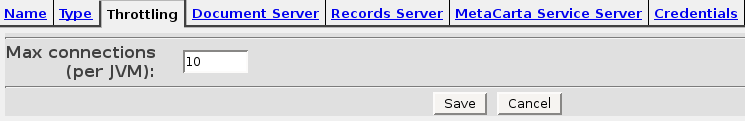
\includegraphics[width=300pt]{mer-edit-auth-tab3}

\begin{itemize}

\item \textbf{Max Connections (per JVM):} The maximum number of
connections per JVM is important for two reasons.
\ifCombinedConnectorGuide \label{max-auth}\fi First, the number of
connections may impact the resources available on your Meridio
server. You should consult your Meridio administrator about an
appropriate maximum number of connections that the crawler may use.

Second, the number of connections may impact the resources available
on the appliance. If the connector framework is slowing down your
appliance, lowering this number should help.

\end{itemize}

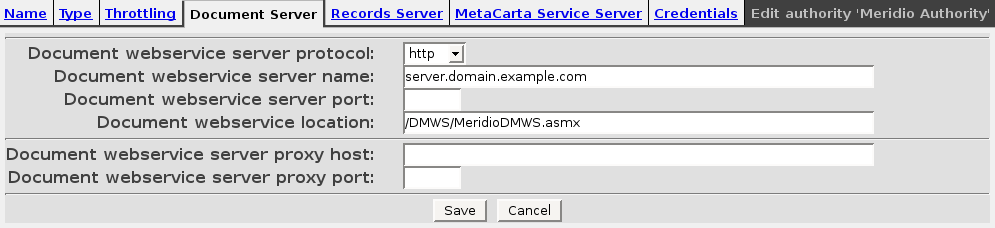
\includegraphics[width=300pt]{mer-edit-auth-tab4}

This tab specifies information about the Meridio document service that
you wish to crawl. You may need to ask your Meridio administrator for
this information.

\begin{itemize}

\item \textbf{Document webservice server protocol:} The appropriate protocol used by your Meridio document webservice, either \texttt{http://} or \texttt{https://}.

\item \textbf{Document webservice server name:} The name of the server hosting your Meridio document webservice.

\item \textbf{Document webservice server port:} The port used to connect to the Meridio document webservice.

\item \textbf{Document webservice location:} The location of the Meridio document webservice on the server specified above. By default, the location of the service is given as \dirpath{/DMWS/MeridioDMWS.asmx}.

\item \textbf{Document webservice server proxy host:} If your MetaCarta appliance must connect to the server hosting the Meridio document webservice using a proxy, specify the name of the appropriate proxy host here.

\item \textbf{Document webservice server proxy port:} The port used to connect to the proxy host.

\end{itemize}

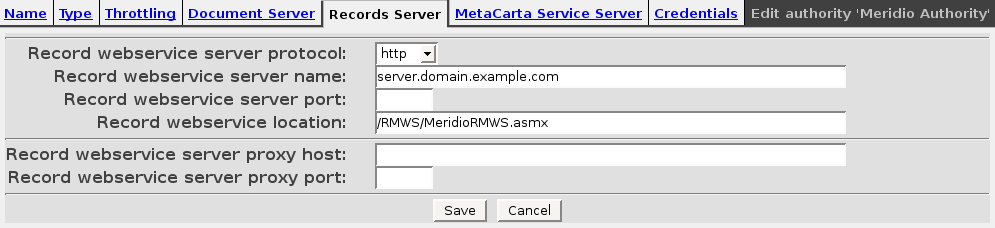
\includegraphics[width=300pt]{mer-edit-auth-tab5}


This tab specifies information about the Meridio record service
corresponding to the document service that you wish to crawl. You may
need to ask your Meridio administrator for this information. Some of
this information may be the same as from the previous tab, as a server
may host more than one Meridio service.


\begin{itemize}

\item \textbf{Record webservice server protocol:} The appropriate protocol used by your Meridio record webservice.

\item \textbf{Record webservice server name:}  The name of the server hosting your Meridio record webservice.

\item \textbf{Record webservice server port:} The port used to connect to the Meridio record webservice.

\item \textbf{Record webservice location:} The location of the Meridio record webservice on the server specified above. By default, the location of the service is given as \dirpath{/RMWS/MeridioRMWS.asmx}

\item \textbf{Record webservice server proxy host:} If your MetaCarta appliance must connect to the server hosting the Meridio record webservice using a proxy, specify the name of the appropriate proxy host here.

\item \textbf{Record webservice server proxy port:} The port used to connect to the proxy host.

\end{itemize}


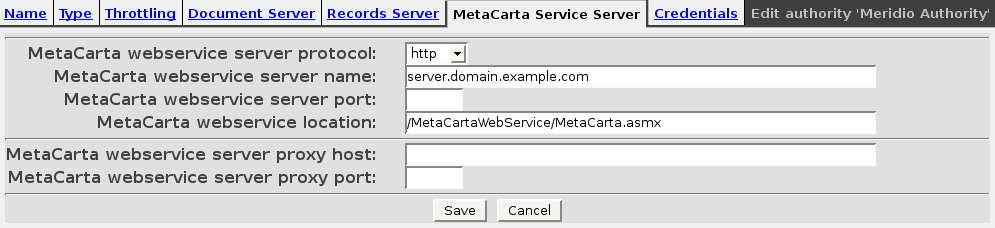
\includegraphics[width=300pt]{mer-edit-auth-tab6}


This tab specifies information about the MetaCarta Meridio Web
Service. See the Installation section, starting on page
\pageref{SWService} for a description of the service and its installation.
The server and service location will be those specified during the
installation of the service. You may need to ask your Meridio
administrator for this information.  Some of this information may be
the same as from the previous tab, as a server may host more than one
Meridio service.


\begin{itemize}

\item \textbf{MetaCarta webservice server protocol:}  The appropriate protocol used by your MetaCarta Meridio Web Service.

\item \textbf{MetaCarta webservice server name:}  The name of the server hosting your MetaCarta Meridio Web Service.

\item \textbf{MetaCarta webservice server port:}  The port used to connect to the MetaCarta Meridio Web Service.

\item \textbf{MetaCarta webservice location:}  The location of MetaCarta Meridio Web Service the on the server specified above. By default, the location of the service is given as \dirpath{/MetaCartaWebService/MetaCarta.asmx}

\item \textbf{MetaCarta webservice server proxy host:}  If your MetaCarta appliance must connect to the server hosting the MetaCarta Meridio Web Service using a proxy, specify the name of the appropriate proxy host here.

\item \textbf{MetaCarta webservice server proxy port:}  The port used to connect to the proxy host.

\end{itemize}



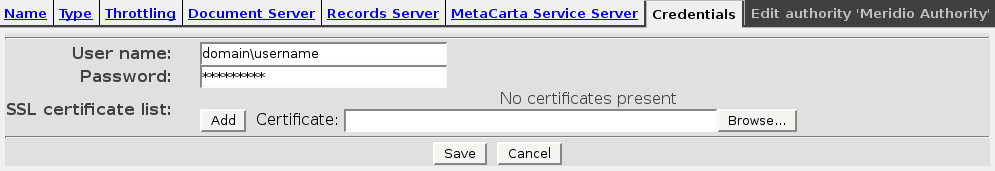
\includegraphics[width=300pt]{mer-edit-auth-tab7}

\begin{itemize}

\item \textbf{User name:} The Active Directory user name that the
appliance should use when connecting to the Meridio services, in the
form \texttt{domain$\backslash{}$username}. This should be an account
created specifically for the appliance.

% Might it be worth a pointer to instructions for doing so?
% Or at least "contact your AD administrator" if that's the right thing?

\item \textbf{Password:} The password for that account.

\item \textbf{SSL certificate list:}
You can upload SSL certificates to use with this connection here. If
you specified ``https'' as the server protocol above, you may need to
upload appropriate certificates or certificate authorities here. The
repository connection will need certificates similar to those used to
connect to your Meridio web service using an Internet browser.


If the certificate authority used to sign your server certificate is a
well-known authority, you will not need to upload a certificate
here. The appliance will automatically accept a certificate from the
server. If the server certificate is signed by an unknown authority,
you should upload the authority's certificate. In some cases, the
authority may be unavailable. In this case, you can upload the
server-side certificate itself. Server-side certificate changes may
require you to upload newer versions of this certificate if you use
this option.


\end{itemize}


After entering this information, you will be taken to the authority
connection status page for this authority:

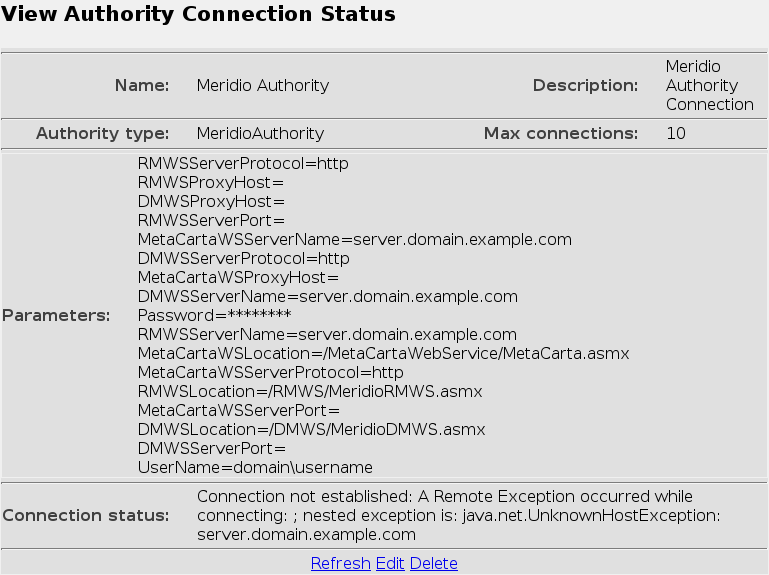
\includegraphics[width=300pt]{mer-view-auth-conn-status}

In this example (which does not contain accurate information for any
Meridio server), the Connection Status is ``Connection not established.''
If you see this message, you may have entered incorrect data into one
of the fields, and should click ``Edit'' to fix the data. If you have
entered everything as you intended, please inform your Meridio
administrator; you may not have been given the correct information,
or one of the services might be down.



\subsection{Creating Repository Connections}

Once you have created an authority connection, you need to create a
repository connection.
To do so, click ``List Repository Connections'' on the sidebar menu. Then,
when presented with the list of repository connections, click ``Add a
new connection.'' You will see the following two tabs:

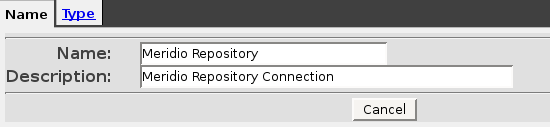
\includegraphics[width=300pt]{mer-edit-repository-tab1}

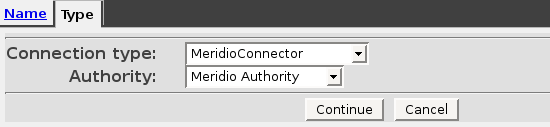
\includegraphics[width=300pt]{mer-edit-repository-tab2}

Now you must provide a name, description, connector type, and
authority type for your new repository connection. The name should be
unique, as you will use it to select this connection later when
defining jobs. The description should explain the repository
connection to you or another administrator.  The connector type is the
type of repository from which you will get documents, in this case a
MeridioConnector. The authority type is the type of authority from
which you will get authorization information. Typically, you will
select the Meridio authority connection that you have set up to
associate with this repository; the permissions associated with the
ingested documents will be the same as the permissions of the original
documents in the Meridio repository. If you intend to force different
Meridio user and group permissions on your documents (see page
\pageref{ForceACL}), then you should select ``Standard (Kerberos)''
here. 

% Can you actually do that with Meridio?

%%% I asked Karl that very question, he said yes.

Once you have filled in those tabs and click continue to move on to
the repository-specific options.

% Licensed to the Apache Software Foundation (ASF) under one or more
% contributor license agreements. See the NOTICE file distributed with
% this work for additional information regarding copyright ownership.
% The ASF licenses this file to You under the Apache License, Version 2.0
% (the ``License''); you may not use this file except in compliance with
% the License. You may obtain a copy of the License at
%
% http://www.apache.org/licenses/LICENSE-2.0
%
% Unless required by applicable law or agreed to in writing, software
% distributed under the License is distributed on an ``AS IS'' BASIS,
% WITHOUT WARRANTIES OR CONDITIONS OF ANY KIND, either express or implied.
% See the License for the specific language governing permissions and
% limitations under the License.

\subsubsection{Configuring a Meridio Repository}

You must fill in the following extra fields if you choose to
configure a Meridio repository connection: 

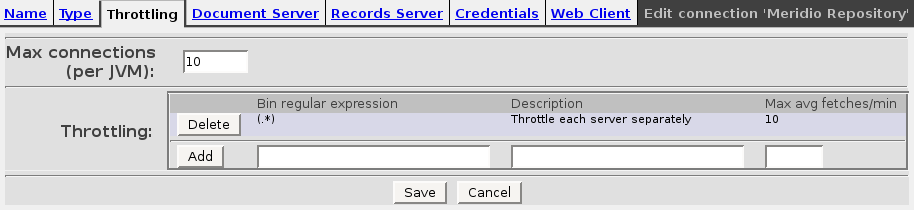
\includegraphics[width=300pt]{mer-edit-repository-tab3}


\begin{itemize}

\item \textbf{Max connections (per JVM):} Here you can set the maximum
number of connections to your repository.

The maximum number of connections per JVM is important for three
reasons.  First, the number of connections may impact the resources
available on your Meridio server. As in the case of the authority
connection, other demands on your Meridio server as well as the
maximum number of conections your server is configured to accept will
influence the number of connections you input here.

Second, the number of connections may impact the resources
available on the appliance. If the connector framework is slowing down
your appliance, lowering this number should help.

Third, only ten document streams can be processed by the appliance at
one time.  If you are also using other repository connectors or the
\command{ingest} command on the appliance, you should reduce this
number to prevent contention for the Ingestion interface. The
Meridio Connector will never overwhelm the interface on its own,
but when other applications are also using the ingestion interface, it
may be best to set the number of repository connections to five or
even fewer.

\item \textbf{Throttling:} Throttling allows you to limit the rate of
document ingestion based on document bin.

The maximum fetch rate allows you to set three things: Expression,
description, and fetches per minute. Each document is part of two
bins: one based on document service and one based on record
service. You can throttle documents from each service individually by
using the expression \texttt{(.*)}, or you can use a blank expression
to throttle all fetches for Meridio crawls together.

% This doesn't make sense to me. So you can only throttle "all fetches" 
% or "these two groups separately?" Why does "pick everything" mean
% "throttle separately?"

\end{itemize}

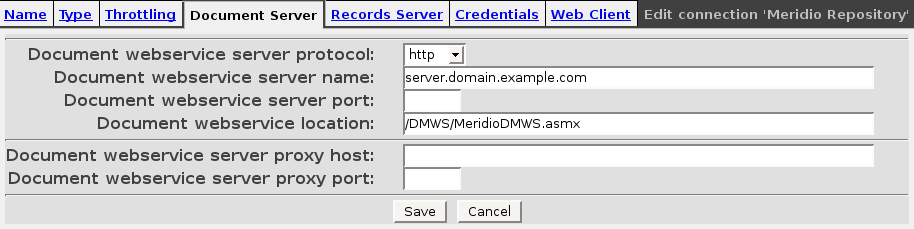
\includegraphics[width=300pt]{mer-edit-repository-tab4}


This tab specifies information about the Meridio document service that
you wish to crawl. You may need to ask your Meridio administrator for
this information. This should be the same information you provided
when creating the Meridio authority connection that you chose to use
with this repository connection.

\begin{itemize}

\item \textbf{Document webservice server protocol:} The appropriate protocol used by your Meridio document webservice.

\item \textbf{Document webservice server name:} The name of the server hosting your Meridio document webservice.

\item \textbf{Document webservice server port:} The port used to connect to the Meridio document webservice.

\item \textbf{Document webservice location:} The location of the Meridio document webservice on the server specified above. By default, the location of the service is given as \dirpath{/DMWS/MeridioDMWS.asmx}.

\item \textbf{Document webservice server proxy host:} If your MetaCarta appliance must connect to the server hosting the Meridio document webservice using a proxy, specify the name of the appropriate proxy host here.

\item \textbf{Document webservice server proxy port:} The port used to connect to the proxy host.

\end{itemize}

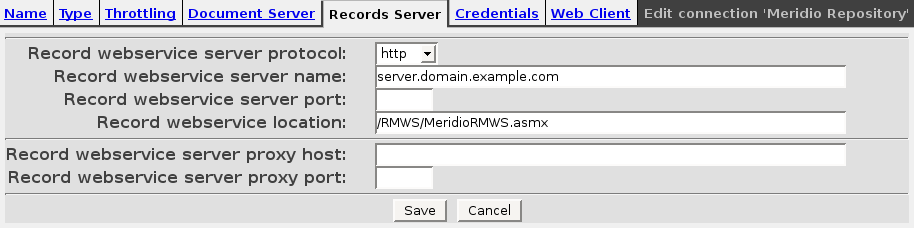
\includegraphics[width=300pt]{mer-edit-repository-tab5}

This tab specifies information about the Meridio record service
corresponding to the document service that you wish to crawl. You may
need to ask your Meridio administrator for this information. Some of
this information may be the same as from the previous tab, as a server
may host more than one Meridio service.  This should be the same
information you provided when creating the Meridio authority
connection that you chose to use with this repository connection.

\begin{itemize}

\item \textbf{Record webservice server protocol:} The appropriate protocol used by your Meridio record webservice.

\item \textbf{Record webservice server name:}  The name of the server hosting your Meridio record webservice.

\item \textbf{Record webservice server port:} The port used to connect to the Meridio record webservice.

\item \textbf{Record webservice location:} The location of the Meridio record webservice on the server specified above. By default, the location of the service is given as \dirpath{/RMWS/MeridioRMWS.asmx}

\item \textbf{Record webservice server proxy host:} If your MetaCarta appliance must connect to the server hosting the Meridio record webservice using a proxy, specify the name of the appropriate proxy host here.

\item \textbf{Record webservice server proxy port:} The port used to connect to the proxy host.

\end{itemize}


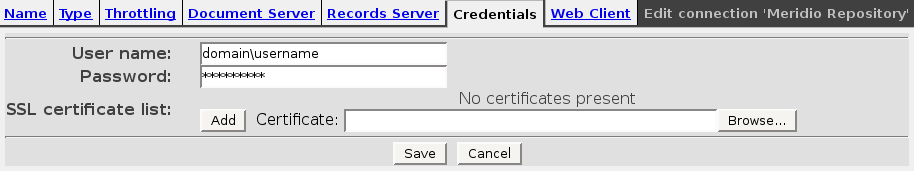
\includegraphics[width=300pt]{mer-edit-repository-tab6}


\begin{itemize}


\item \textbf{User name:} The Active Directory user name that the appliance should use when connecting to the Meridio services, in the form \texttt{domain$\backslash{}$username}. This should be an account created specifically for the appliance that you specified when creating the corresponding authority connection.

\item \textbf{Password:} The password for that account.

\item \textbf{SSL certificate list:}
You can upload SSL certificates to use with this connection here. If
you specified ``https'' as the server protocol above, you may need to
upload appropriate certificates or certificate authorities here. The
repository connection will need certificates similar to those used to
connect to your Meridio web service using an Internet browser.


If the certificate authority used to sign your server certificate is a
well-known authority, you will not need to upload a certificate
here. The appliance will automatically accept a certificate from the
server. If the server certificate is signed by an unknown authority,
you should upload the authority's certificate. In some cases, the
authority may be unavailable. In this case, you can upload the
server-side certificate itself. Server-side certificate changes may
require you to upload newer versions of this certificate if you use
this option.



\end{itemize}


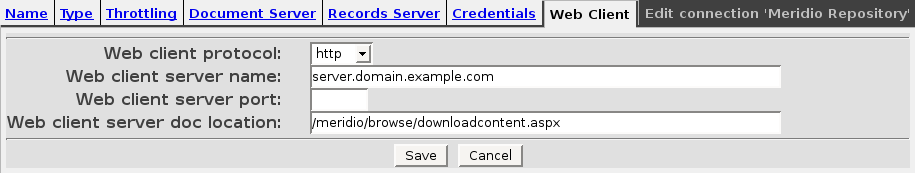
\includegraphics[width=300pt]{mer-edit-repository-tab7}

This tab specifies information about the web client service that can
be used to view the documents and records that are being processed by
the crawler. The information you provide here is used by the appliance
to generate retrieval URLs that are shown to appliance users. You may
need to ask your Meridio administrator for this information. Some of
this information may be the same as from previous tabs, as a server
may host more than one Meridio service.

\begin{itemize}

\item \textbf{Web client server protocol:}  The appropriate protocol used by your Meridio web client service.

\item \textbf{Web client server name:}  The name of the server hosting your Meridio web client service.

\item \textbf{Web client server port:}  The port used to connect to the Meridio web client service.

\item \textbf{Web client server doc location:}  The location of the Meridio web client service on the server specified above. By default, the location of the service is given as \dirpath{/meridio/browse/downloadcontent.aspx}.

\end{itemize}

After entering this information, you will be taken to the status page
for this repository connection:

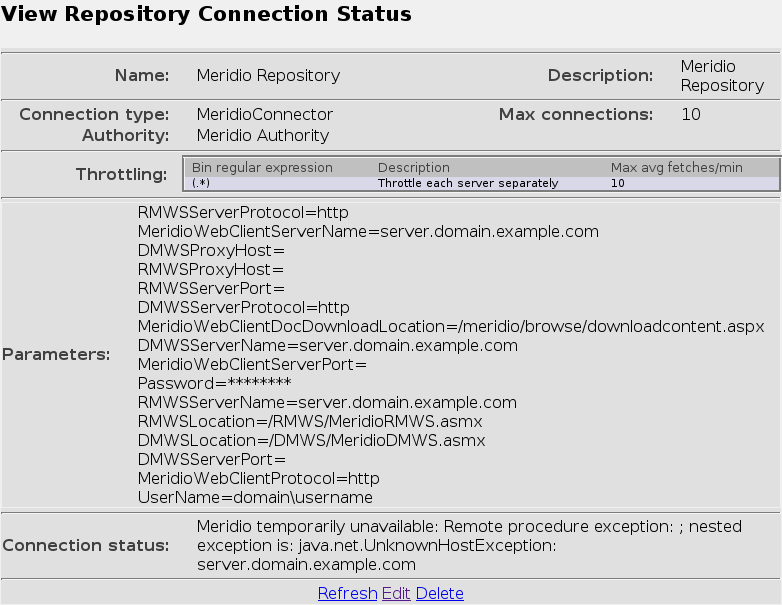
\includegraphics[width=300pt]{mer-view-repo-conn-status}

In this example (which does not contain accurate information for
any Meridio server), the Connection Status is ``Meridio temporarily
unavailable.''  If you see this message, your Meridio services may not be
responding, or you might have incorrectly entered one of the fields, and
should click ``Edit'' to fix the data. If you have entered everything as
you intended,  and the Meridio services are up, please inform your Meridio
administrator; you may not have been given the correct information.



\subsection{Creating and Running Jobs}

To run a job, click ``Status and Job Management'' on the sidebar menu.
You can run or edit existing jobs from this menu.

To create a new job, click ``List All Jobs'' on the sidebar menu. Then, when
presented with the list of current jobs, click ``Add a new job.'' You
will be presented with two tabs, in which you must fill in the following
information:

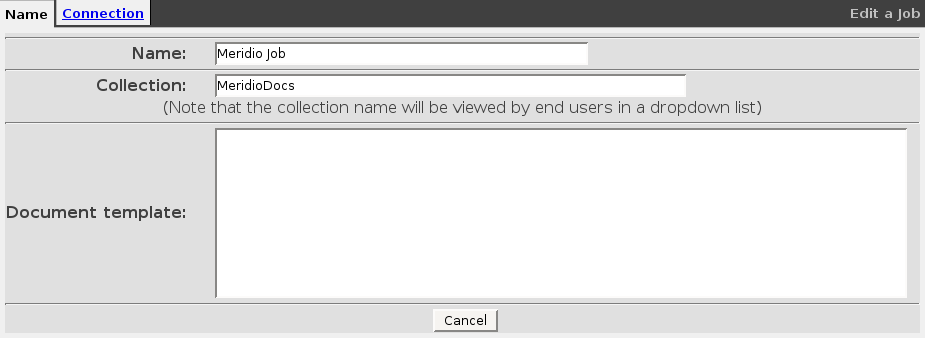
\includegraphics[width=300pt]{mer-edit-job-tab1}

\begin{itemize}

\item \textbf{Name:} The name of the job. You will use this to identify
the job later.

\item \textbf{Collection:} The collection name metadata for all
documents in this job. End users can use this name to select the set
of documents in this job. For more information on collection name
metadata, please see the \documentref{MetaCarta GTS Administrator's
Guide}.

\item \textbf{Document template:} % Licensed to the Apache Software Foundation (ASF) under one or more
% contributor license agreements. See the NOTICE file distributed with
% this work for additional information regarding copyright ownership.
% The ASF licenses this file to You under the Apache License, Version 2.0
% (the ``License''); you may not use this file except in compliance with
% the License. You may obtain a copy of the License at
%
% http://www.apache.org/licenses/LICENSE-2.0
%
% Unless required by applicable law or agreed to in writing, software
% distributed under the License is distributed on an ``AS IS'' BASIS,
% WITHOUT WARRANTIES OR CONDITIONS OF ANY KIND, either express or implied.
% See the License for the specific language governing permissions and
% limitations under the License.

You may also input a document template. A document template, written
in XML, limits the parts of the document that are indexed.  Simply
input the XML in the text entry field.  For information on how to
construct a document template, please see the \documentref{MetaCarta
Document Templates Integrator's Guide}.


\end{itemize}

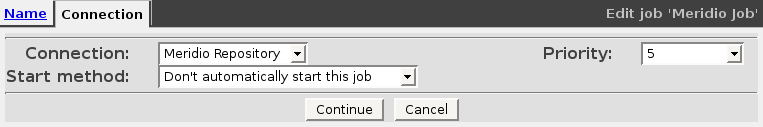
\includegraphics[width=300pt]{mer-edit-job-tab2}

\begin{itemize}

\item \textbf{Connection:} The name of the repository connection you
wish to use for this job. You select this from the list of repository
connections you have already made. You may have more than one job
use the same repository connection, but if you have two jobs crawl the
same documents, the documents will have the metadata and collection name
associated with whatever job crawled the document most recently. This will
cause unpredictable results for end users searching those collections
or searching for those documents, or administrators trying to delete
those collections.  We recommend never crawling the same document in
two different jobs.

\item \textbf{Start method:} Whether you want to start this job the next
time jobs are scheduled to run (``Start when schedule window starts''),
immediately after you finish defining it (``Start even inside a schedule
window''), or not at all (``Don't automatically start this job'').

\item \textbf{Priority:} From 1 (highest) to 10 (lowest), the priority
this crawl should have if it must compete for resources with other
crawls on the appliance. You should not need to change this unless you
are running more than one crawl at the same time; if you are, assign a
higher priority to the crawls whose documents you want to be processed
preferentially before documents from other jobs.

\end{itemize}

After filling in those options, click ``Continue,'' and you will be
presented with seven additional repository-specific tabs. 

% Licensed to the Apache Software Foundation (ASF) under one or more
% contributor license agreements. See the NOTICE file distributed with
% this work for additional information regarding copyright ownership.
% The ASF licenses this file to You under the Apache License, Version 2.0
% (the ``License''); you may not use this file except in compliance with
% the License. You may obtain a copy of the License at
%
% http://www.apache.org/licenses/LICENSE-2.0
%
% Unless required by applicable law or agreed to in writing, software
% distributed under the License is distributed on an ``AS IS'' BASIS,
% WITHOUT WARRANTIES OR CONDITIONS OF ANY KIND, either express or implied.
% See the License for the specific language governing permissions and
% limitations under the License.

\subsubsection{Meridio Job Options}

You must fill in the following extra fields if you are configuring a
Meridio job:

\bigimage{mer-edit-job-tab3}

% Licensed to the Apache Software Foundation (ASF) under one or more
% contributor license agreements. See the NOTICE file distributed with
% this work for additional information regarding copyright ownership.
% The ASF licenses this file to You under the Apache License, Version 2.0
% (the ``License''); you may not use this file except in compliance with
% the License. You may obtain a copy of the License at
%
% http://www.apache.org/licenses/LICENSE-2.0
%
% Unless required by applicable law or agreed to in writing, software
% distributed under the License is distributed on an ``AS IS'' BASIS,
% WITHOUT WARRANTIES OR CONDITIONS OF ANY KIND, either express or implied.
% See the License for the specific language governing permissions and
% limitations under the License.

\begin{itemize}
\label{scheduling}

\item \textbf{Schedule type:} Whether you want to scan every document
once or dynamically recrawl content in your repository. 

When scanning every document once, the crawler marks all documents that
have been previously crawled in this job as potentially to be deleted,
adds all seed documents to its queue and marks them as pending, processes
pending documents, marking them completed as they are ingested, and then
deleted all of the documents that were not recrawled. A document might
not be recrawled because it no longer exists, or the job specification
might have been changed to no longer include the document.

When dynamically recrawling documents, the crawler does not start by
marking all documents as potentially deletable; instead, it begins with
all of the seed documents, and continues adding to its list, periodically
re-adding the initial seed documents. If a document is removed from the
source, it will expire in the expiration interval (see below).

\item \textbf{Expiration Interval (if continuous):} The length of the
interval (in minutes) that the appliance will retain a document
crawled by this job after the document no longer appears in the
repository. After this interval, the missing document will be removed
from the appliance's index and archive. Leave the expiration interval
blank to keep missing documents indexed in GTS.

\item \textbf{Recrawl interval:} If you are dynamically recrawling
documents, how long, in minutes, the crawler should wait before
crawling documents a second time.

\item \textbf{Reseed interval:} If you are dynamically recrawling
documents, how long, in minutes, the crawler should wait before
looking for new documents to crawl. \ifMeridioGuide This connector
identifies all documents for ingestion through seeding; if the reseed
interval is infinite, the job will not ingest documents placed in the
repository during run time. (The job automatically reseeds whenever it
is started.) The default interval of 60 minutes is an appropriate
reseed rate. \fi \ifFilenetGuide This connector identifies documents
for ingestion during seeding. If you change the document inclusion
criteria, reseeding is required to identify new documents. Similarly,
documents placed in the repository while the job is running will not
be identified until the crawl is reseeded.  (The job automatically
reseeds whenever it is started.) The default interval of 60 minutes is
an appropriate reseed rate. \fi

\item \textbf{Scheduled time:} Allows you to define a time you wish
the job to run using a series of selection boxes. The first box refers
to the day of the week you wish the job to run, with an option to have
the job run any day of the week. The second box allows you to select
the start hour, with an option to start the job at any hour. The third
box allows you to specify which minute after the hour that you wish
the job to start. The fourth box allows you to specify what months of
the year you wish the job to run, with an option for the job to run
any month. The last box allows you to specify the day of the month you
wish the job to start, including any day of month.


You can scroll through each of the five boxes in this setting using
the arrow keys on your keyboard or by using the scroll bar on the
right side of the box.  If you want to select more than one value,
hold down control as you scroll and click the values that you want to
select. This allows you to define multiple windows with the same
length, for example by selecting Monday, Wednesday, and Friday at the
same time.

\item \textbf{Maximum run time:} The longest you will allow the job to
run, in minutes. For example, if you want to start a job at 2 AM but
force it to stop at 8 AM so that users have access to the repository,
you should set this value to 360 minutes. If the job is not complete by the
end time, documents that have already been found will be indexed, and
the rest of the crawl will continue at the beginning of the next
schedule interval. 

When you have defined the scheduled time and assigned a maximum run
time, click on the ``Add Scheduled Time'' button. A new schedule box
will appear below the scheduled time, allowing you to create
additional scheduled run times.

Here is a sample schedule for a job that will run every
Monday from 2 am to 6 am:

\begin{changemargin}{-.3in}{0in} 
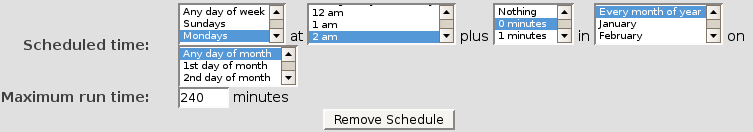
\includegraphics[width=300pt]{sample-schedule}
\end{changemargin}

If you do not have at least one scheduled time, the job will
only run when run manually (see page \pageref{ManageJobs}), and will
not automatically update the index on the appliance based on changes
to the repository.

You can remove a scheduled time by clicking the ``Remove Schedule''
button.

\end{itemize}


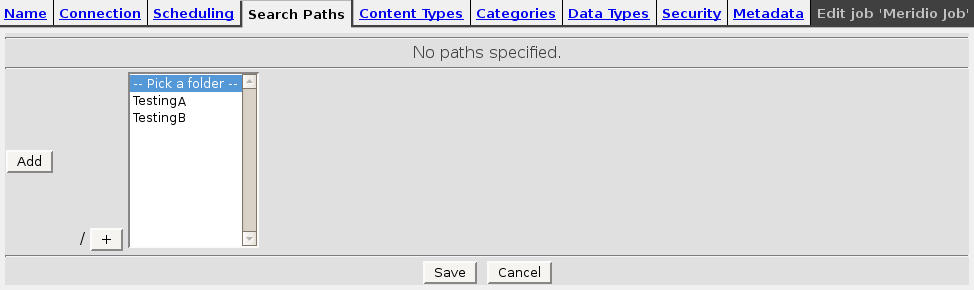
\includegraphics[width=300pt]{mer-edit-job-tab4}

\begin{itemize}

\item \textbf{Paths:} The directory paths in your Meridio
service from which you want your crawl to start. You can specify
one or more directory paths. If you do not specify directory paths,
the job will crawl all directories in your Meridio service. You
can build directory paths by selecting individual directories. To
start, select the base directory of the path you wish to create, then
click the ``+'' button. A new selection box will appear with the
directories contained by that parent directory. Select a directory at
that level and click the ``+'' button. Continue building your
directory path in this fashion. When it's complete, click ``Add''. A
new selection box will appear beneath the added directory path. You
can continue to add more directory paths to your list. To remove a
directory path from the list, click the ``Delete'' button next to it.

\end{itemize}

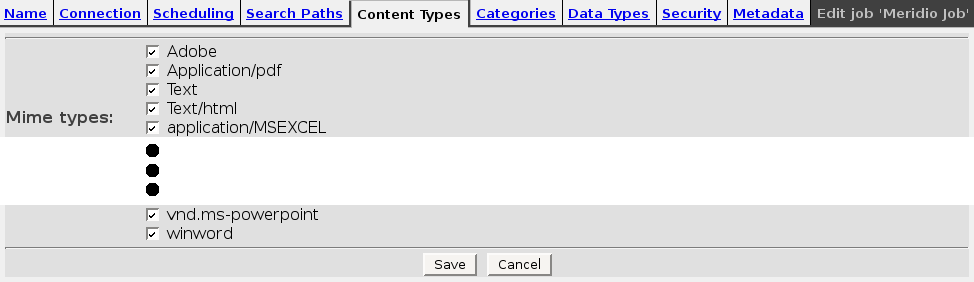
\includegraphics[width=300pt]{mer-edit-job-tab5}

\begin{itemize}

\item \textbf{Mime Types:} Check the
mime types you wish to include in this job. This list of mime types is
based on the mime types that the appliance is capable of ingesting.

\end{itemize}

%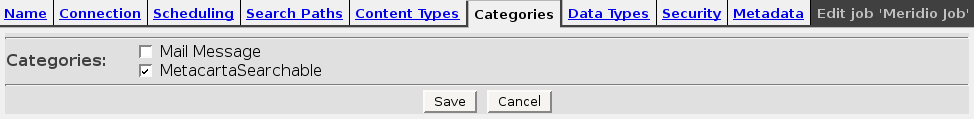
\includegraphics[width=300pt]{mer-edit-job-tab6}

\begin{itemize}

\item \textbf{Categories:} Check the categories that you wish to include in this job. These categories are created by your Meridio administrator; ask your administrator which categories you should include.

\end{itemize}

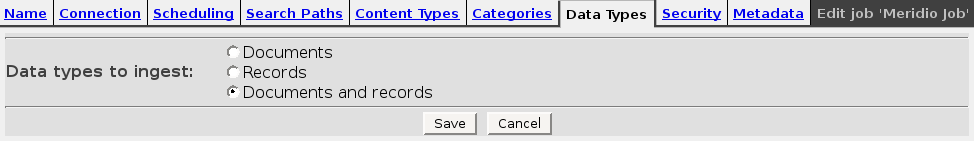
\includegraphics[width=300pt]{mer-edit-job-tab7}

\begin{itemize}

\item \textbf{Data types to ingest:} 
Here you can specify if this job should include \textbf{Documents},
\textbf{Records}, or \textbf{Documents and records}.
 
\end{itemize}


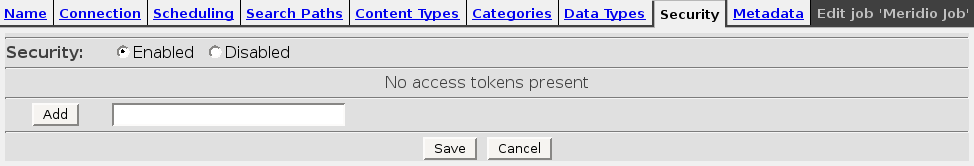
\includegraphics[width=300pt]{mer-edit-job-tab8}

\begin{itemize}

\item \textbf{Security:} Use this option to enable or disable document
security. If you choose to enable security, user permissions will be
ingested with documents, while if you choose to disable security,
documents will be ingested without permissions.

\item \textbf{Access Tokens:} \label{ForceACL} If you wish to specify
your own permissions lists for files ingested through this job, you
can specify them here. You should use this option if you selected
``Standard (Kerberos)'' as the authority connection for your
repository connection and you are choosing to enable security. Simply
enter one or more Meridio user or group identifiers into the field and
click the ``Add'' button. The identifiers will appear in a list. You
can continue to add more identifiers using the ``Add'' button, or
remove them using the ``Delete'' button that appears next to each
identifier.

\end{itemize}

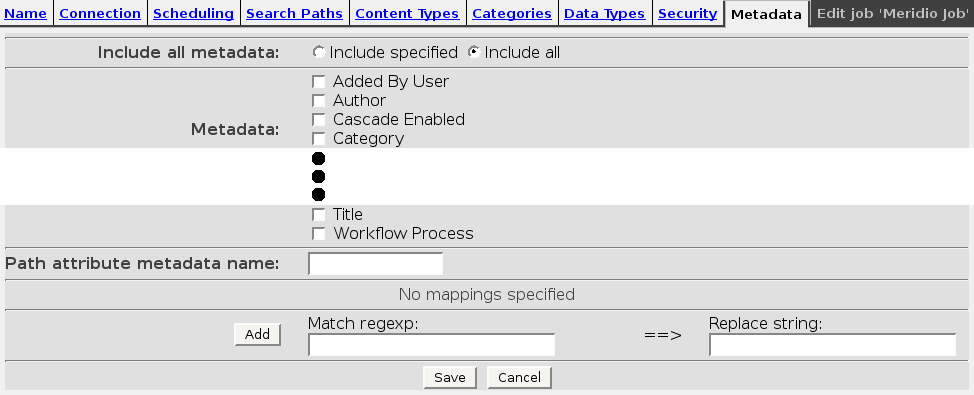
\includegraphics[width=300pt]{mer-edit-job-tab9}

\begin{itemize}

\item \textbf{Include all metadata:} This allows you to chose between including all metadata present for each file and creating a subset of the metadata attributes to include. If you select ``Include specified'', you can use the following field to select the metadata attributes you want to include.

\item \textbf{Metadata:} Each metadata field that is available on your Meridio system is listed here.

\item \textbf{Path attribute metadata name:} The Meridio Connector does not support path attribute metadata. Leave this field blank.

\item \textbf{Path-value mapping:} Leave these fields blank.

\end{itemize}


After entering this information, you will be taken to the status page
for this job:

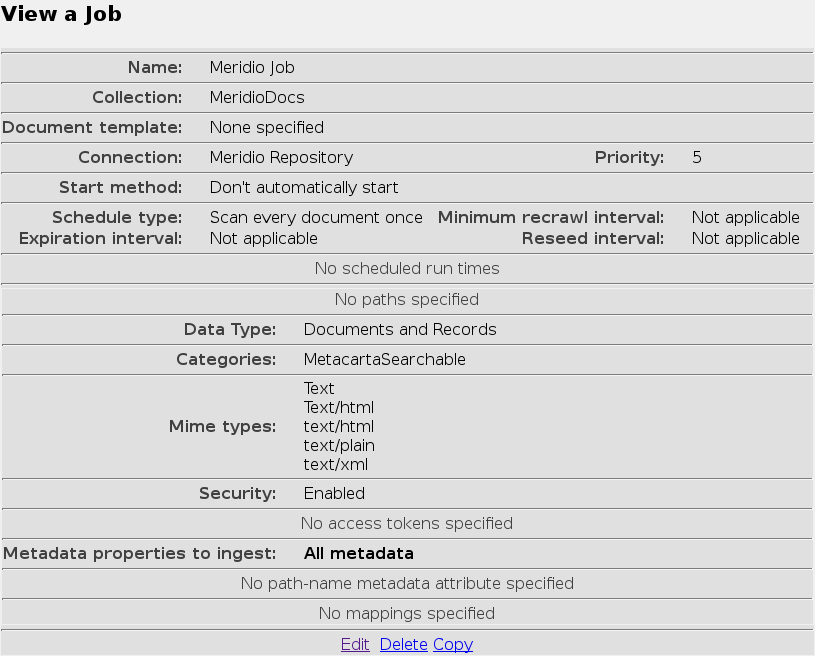
\includegraphics[width=300pt]{mer-view-job-status}



\subsection{\label{ManageJobs}Status and Job Management}

You can then look at the status of your job by clicking ``Status and 
Job Management'' on the sidebar. You will see a list of one or more jobs
much like this one:

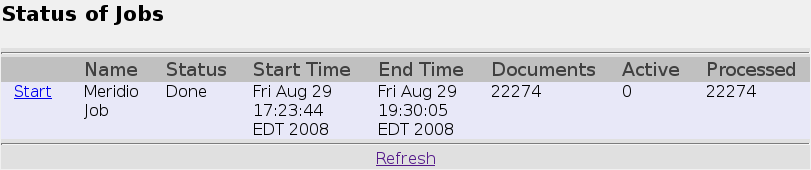
\includegraphics[width=300pt]{mer-jobs-list}

You can start any crawl you like immediately from this interface by
clicking ``Start'' next to the name of the crawl. This interface also
allows you to see how many documents have been crawled; this information
may help you structure and plan future crawls.

\note{Refresh this page by clicking the ``Refresh'' link at the bottom
of the page, not by clicking your browser's reload button.}

\section{Reports}

The Connector interface can generate two types of status reports, on
current crawl status, and four types of history reports, on past crawl
history.

\subsection{Status Reports}

The two types of status report are:

\begin{itemize}

\item Document Status, which lets you find information on individual
documents currently part of a job.

\item Queue Status, which lets you aggregate information about groups
of documents currently part of a job.

\end{itemize}

\subsubsection{Document Status}

This report was generated by selecting ``Meridio Repository
Connection,'' selecting the document state ``Documents processed at
least once,'' selecting all possible document statuses, clicking
continue, selecting ``Meridio Job,'' and clicking Go.

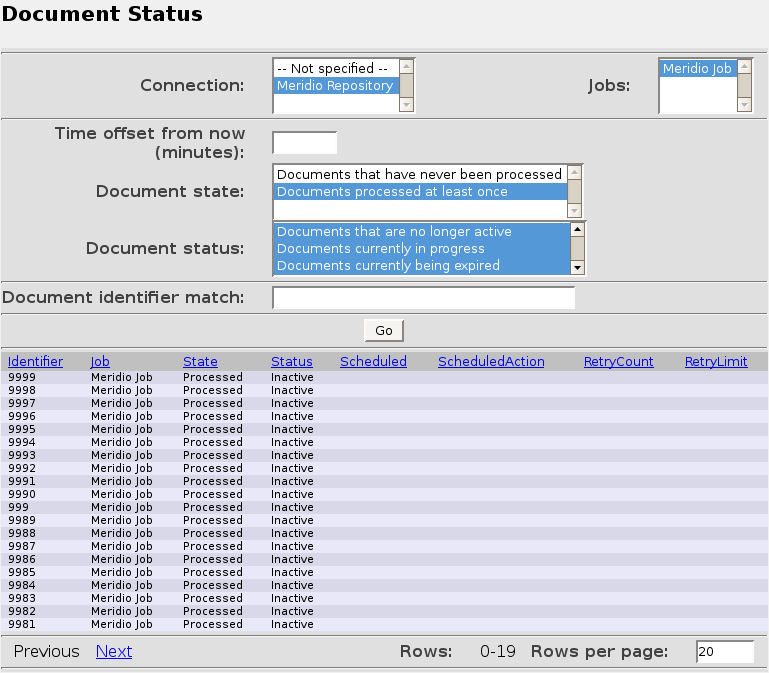
\includegraphics[width=300pt]{mer-document-report}

\begin{itemize}

\item \textbf{Connection:} The repository connection from which to 
generate a report. You must select the repository connection and click
Continue to see all repository-specific options. %Are there any?

\item \textbf{Time offset from now:} Defaults to zero. Allows you to
see estimates of future status or, with negative numbers, a record of
past status.

\item \textbf{Document state:} Allows you to select documents that
have not yet been processed or documents that have been processed
at least once.

\item \textbf{Document status:} Allows you to choose one or more 
statuses of document to report on. The statuses you can choose are:

\begin{itemize}

\item Documents that are no longer active

\item Documents currently in progress

\item Documents currently being expired

\item Documents currently being deleted

\item Documents currently available for processing

\item Documents currently available for expiration

\item Documents not yet processable

\item Documents not yet expirable

\end{itemize}

\item \textbf{Document identifier match:} A regular expression
allowing you to see only documents with matching identifiers. Meridio
document identifiers are typically numbers. To see all documents, use
a blank matching expression. Other possible match expressions include:

\begin{itemize}

\item \textbf{\^{}1}: Only documents whose identifiers begin with \texttt{1}.

\item \textbf{234}: Only documents whose identifiers contain the
string \texttt{234}.

\item \textbf{[1,2]\$}: Only documents whose identifiers end in
\texttt{1} or \texttt{2}.

\end{itemize}

\note{If you are not familiar with regular expressions, \label{regex}
there are a variety of tutorials available on the web,
including \url{http://gnosis.cx/publish/}\linebreak
\url{programming/regular_expressions.html} and
\url{http://perldoc.}\linebreak\url{perl.org/perlrequick.html}. If you
still have difficulty with these settings, please contact Customer Support
(see page \pageref{SupportContact}).}


\item \textbf{Jobs:} The job or jobs for which you want to generate
a report.

\end{itemize}

You can sort this report by any of the returned fields; to do so,
click the field names.

\subsubsection{Queue Status}

This report was generated by selecting ``Meridio Repository
Connection,'' selecting both document states, selecting all possible
document statuses, clicking continue, selecting ``Meridio Job,''
setting the identifier class description to \texttt{([0-9])\$}, and
clicking Go.

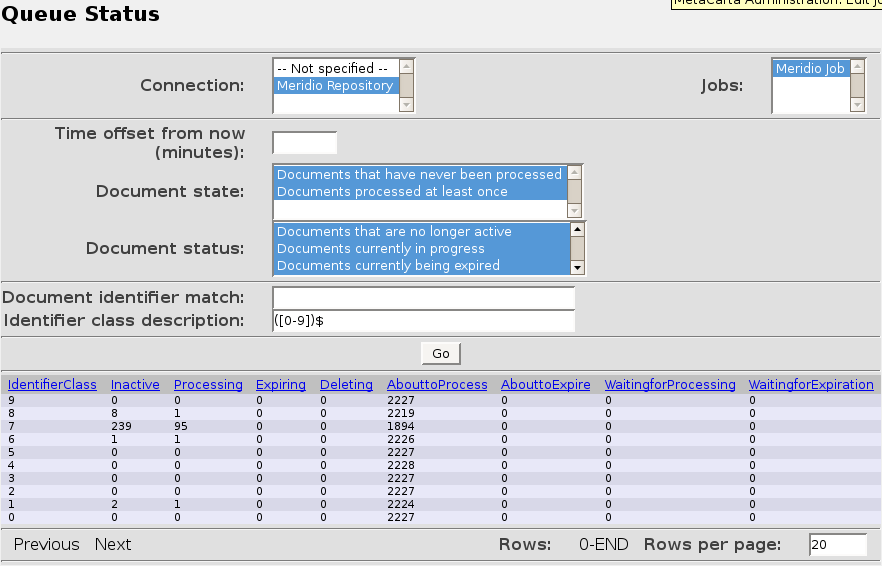
\includegraphics[width=300pt]{mer-queue-report}

This form offers the same fields as the Document Status report with
one addition, the \textbf{Identifier class description}, which allows
you to group results based on a regular expression. In this case,
documents are grouped together based on their last digit. The
ungrouped documents are all analyzed together in the first row of the
table. Other possibilities would be \texttt{(.*)}, which would put
each document in a group alone, or \texttt{\^{}(1)}, which would group
together all documents with the first digit \texttt{1}.  In this
second case, all ungrouped documents would be analyzed together in the
first row of the table.

\subsection{History Reports}

The four types of history report are:

\begin{itemize}

\item Simple History, which lets you list an ordered set of log events
based on chosen criteria

\item Maximum Activity, which lets you see the period of time in
which a certain event happened most often

\item Maximum Bandwith, which lets you see the period of time in
which the most bandwidth was used 

\item Result Histogram, which provides log information that would be
appropriate for constructing a histogram or other diagram

\end{itemize}

Each of these reports allows you to specify a connection, one or more
activities, a start time, an end time, an entity match, and a result code
match.  Some also allow you to specify an identifier class description
and a sliding window size. This section will show sample results for
each type of report and an explanation of the fields selected.

\subsubsection{Simple History}

This report was generated by selecting ``Meridio Repository Connection,'' 
clicking Continue, selecting ``document ingest,'' and clicking Go.

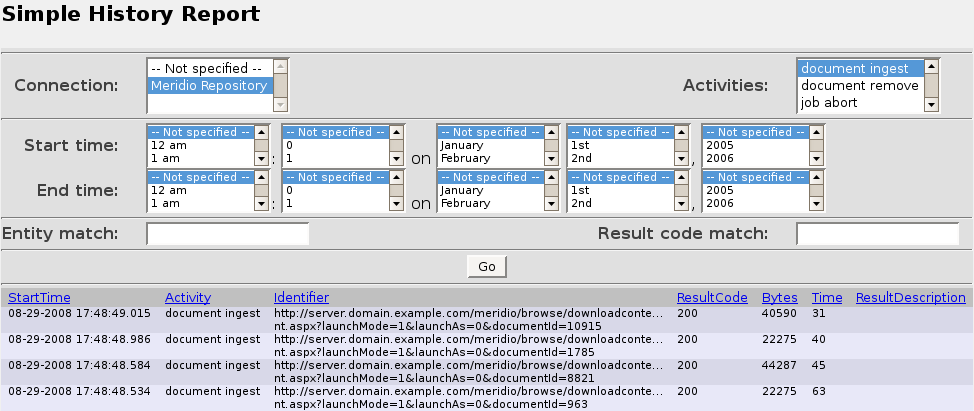
\includegraphics[width=300pt]{mer-simple-history-report}

\begin{itemize}

\item \textbf{Connection:} The repository connection from which to generate
a report.

\item \textbf{Activities}: What crawler activities you would like to
see.  Your options are document ingest, document remove, job
abort, job continue, job end, job start, and job wait.

\item \textbf{Start time}: The earliest time in the crawler logs to be
considered for this query.  Choose ``Not specified'' for any field to
start at the beginning of the crawler's logs.

\item \textbf{End time:} The latest time in the crawler logs to be
considered for this query. Choose ``Not specified'' for any field 
to end at the current time.

\item \textbf{Entity match:} A regular expression to limit the
Identifier field. In this case, the document identifier will be the
URL created for document retrieval, with the only unique portion being
the document identification number.
If the entity match field in the example above had
been \texttt{17\$}, only document fetches with identifiers ending
with 17 would be shown. For more assistance with regular expressions, see the note on page \pageref{regex}.

\item \textbf{Result code match:} A regular expression to limit the
ResultCode field.

\end{itemize}

You can sort the history report by any of the returned fields; to do so,
click the field names.

\subsubsection{Maximum Activity}

This report was generated by selecting ``Meridio Repository
Connection,'' clicking Continue, selecting ``document ingest,''
changing the Entity match and Identifier class description, and
clicking Go.

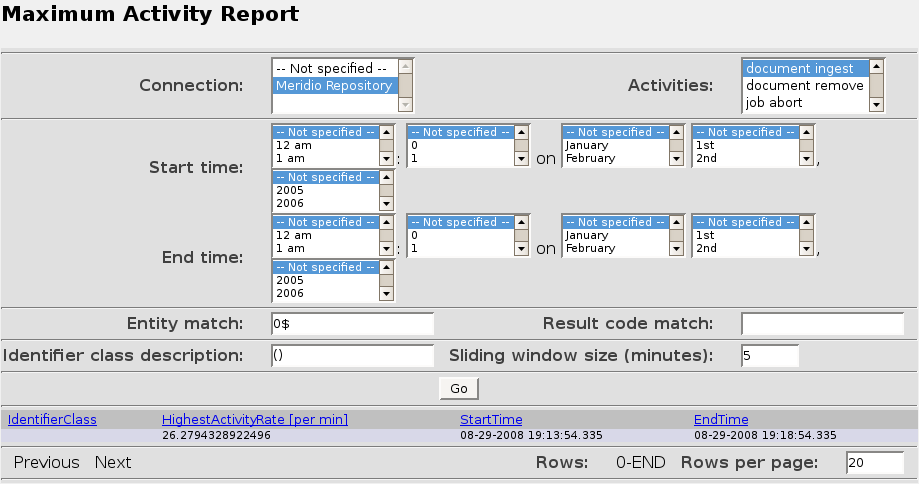
\includegraphics[width=300pt]{mer-maximum-activity-report}

This form offers two more fields than the previous form:

\begin{itemize}

\item \textbf{Identifier class description:} A regular expression that
determines how to group identifiers together. If this were set to
\texttt{(.*)}, there would be no grouping, and so there would be only
one ingestion event per document. If this were set to
\texttt{([0-9])\$}, then all documents with identifiers ending with
the same digit would be grouped together. The setting in the example,
\texttt{()}, groups all documents together. Some other possibilities:

\item \textbf{Sliding window size}: The search interval in minutes.

\end{itemize}

The report returned will have only one result per group with one or more
documents in it, if there is a clear highest activity rate, or a list of
all the results tied for highest activity rate if there are more than one.

\subsubsection{Maximum Bandwidth}

This report was generated by selecting ``Meridio Repository
Connection,'' clicking Continue, selecting ``document ingest,''
changing the Entity match and Identifier class description, and
clicking Go.

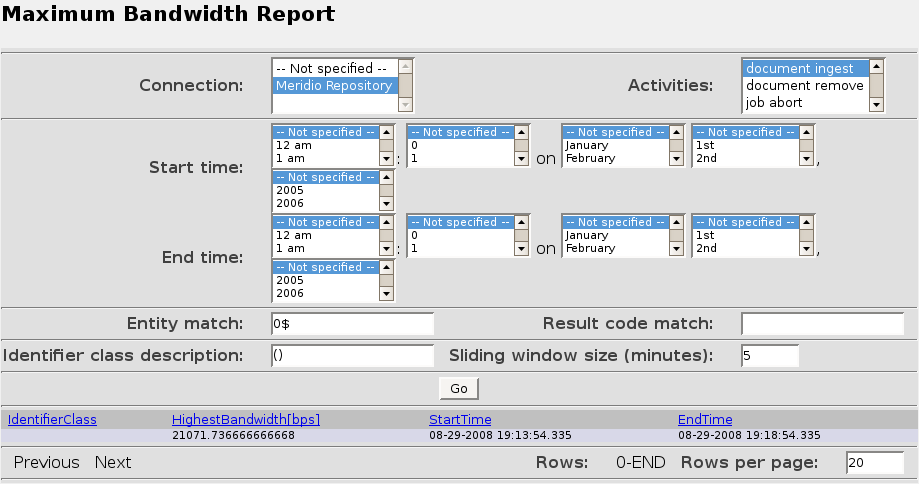
\includegraphics[width=300pt]{mer-maximum-bandwidth-report}

This form offers the same fields as the maximum activity form, and
returns similar results; instead of tracking events per time window,
it tracks the window with the highest average bandwith usage, measured
in bytes per second. Again, the identifier class description has been
changed to a regular expression that will match all identifiers (and
thus in this case all documents).

\subsubsection{Result Histogram}

This report was generated by selecting ``Meridio Repository
Connection,'' clicking Continue, selecting ``document ingest,'' and
clicking Go.

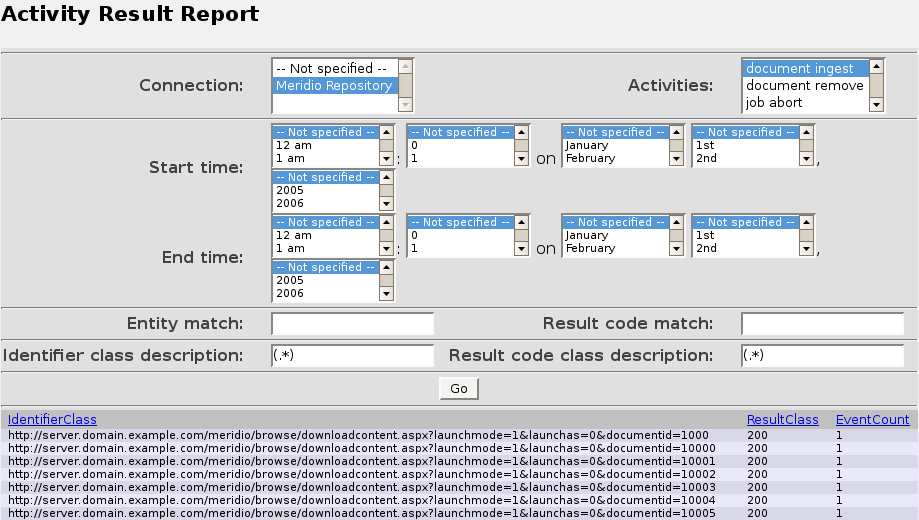
\includegraphics[width=300pt]{mer-activity-result-report}

This form adds one new field:

\begin{itemize}

\item \textbf{Result code class description:} A regular expression that
determines how to group result classes together; like Identifier class
descriptions but for result classes.

\end{itemize}

This report does not produce an actual histogram, but provides data that
could be used to generate histograms.  
 
\end{changemargin}
